\documentclass{article}[18pt]
\usepackage[utf8]{inputenc}
\usepackage[margin=0.7in]{geometry}
\usepackage{parselines} 
\usepackage{amsmath}
\usepackage{titlesec}
\usepackage{pgfplots}
\usepackage{graphicx}
\usepackage[english]{babel}
\usepackage{fancyhdr}
\usepackage{gensymb}

\pgfplotsset{width=10cm,compat=1.9}

\titlespacing\section{0pt}{14pt plus 4pt minus 2pt}{0pt plus 2pt minus 2pt}
\newlength\tindent
\setlength{\tindent}{\parindent}
\setlength{\parindent}{0pt}
\renewcommand{\indent}{\hspace*{\tindent}}
\pretolerance=10000
\hyphenpenalty=10000
\pagestyle{fancy}
\fancyhf{}
\rhead{Sam Robbins 13SE}
\lhead{A Level Maths - M2}
\rfoot{Page \thepage}


\begin{document}
\begin{center}
\underline{\huge Collisions}
\end{center}
\section{Impulse and momentum}
Impulse=$mv-mu$=$Ft$\\
Total momentum before collision=total momentum after
\section{Coefficient of restitution}
This tells us how well something bounces, it is given the symbol \textbf{e}.\\
If $e=1$ the ball returns to it's original height\\
If $e=0$ the ball doesn't bounce\\
\\
$e=\dfrac{\text{Speed of seperation}}{\text{Speed of approach}}$
\subsection{Alternate form of coefficient of restitution formula}
$mgh=\frac{1}{2}mv^2$\\
\\
$v=\sqrt{2gh}$\\
\\
$e=\dfrac{\sqrt{2gh_2}}{\sqrt{2gh_1}}$\\
\\
$e=\dfrac{\sqrt{h_2}}{\sqrt{h_1}}$\\
\\
$h_2$ - the height the ball bounces back to\\
\\
$h_1$ - the height the ball is dropped from
\subsection{Calculations involving coefficient of restitution}
When doing calculations involving the coefficient of restitution both the calculation for CoR and conservation of momentum will be needed.\\
\textbf{Conservation of momentum:}
$m_1u_1+m_2u_2=m_1v_1+m_2v_2$\\
\\
\textbf{Coefficient of restitution}\\
\\
$e=\dfrac{v_1}{u_1}$
\subsection{Successive Impacts}
In some cases calculations will involve the impacts of multiple balls successively, like in newton's cradle.
\subsubsection{Example}
\textit{Three perfectly elastic particles A, B and C with masses 3kg, 2kg and 1kg respectively lie at rest in a straight line on a smooth horizontal table in alphabetical order. A is projected towards B with speed $5ms^{-1}$ and after A has collided with B, B collides with C}\\
\\
$5\times3=3V_A+2V_B$\\
\\
$1=\dfrac{SoS}{SoA}$ therefore $SoS=SoA$ so $V_B-V_A=5$ so $V_B=5+V_A$\\
\\
$15=10+2V_A+3V_A$\\
\\
$15=2V_B+3$ so after 1st collision $V_B=6$\\
\\
$15=10+5V_A$ so $\mathbf{V_A=1}$\\
\\
\textbf{2nd Collision}\\
\\
$2\times6=2V_B+V_C$\\
\\
$V_C-V_B=6$\\
\\
$12=3V_B+6$\\
\\
$3V_B=6$\\
\\
$\mathbf{V_B=2}$\\
\\
$V_C=6+2=8$
\newpage
\begin{center}
\underline{\huge Collisions example - Direct Impact}
\end{center}
\textit{A small ball A of mass 3m is moving with speed u in a straight line on a smooth horizontal
table. The ball collides directly with another small ball B of mass m moving with speed u
towards A along the same straight line. The coefficient of restitution between A and B is $\frac{1}{2}$
The balls have the same radius and can be modelled as particles.}\\
\\
\textit{Find the speed of A immediately after the collision}\\
\\
\\
\textbf{1. Draw the diagram in its initial state}\\
\\
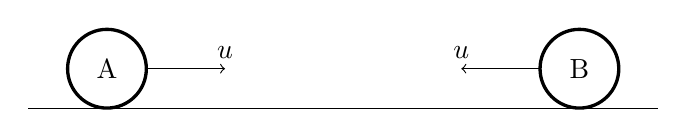
\begin{tikzpicture}
\filldraw[color=black,fill=none,very thick](3,0.5) circle (0.5) node{B};
\filldraw[color=black,fill=none,very thick](-3,0.5) circle (0.5) node{A};
\draw (-4,0) -- (4,0);
\draw[arrows=->](-2.5,0.5)--(-1.5,0.5) node[above]{$u$};
\draw[arrows=->](2.5,0.5)--(1.5,0.5) node[above]{$u$};
\end{tikzpicture}\\
\\
\textbf{2. Apply the conservation of momentum formula (make sure to remember different directions)}\\
\textcolor{red}{$m_1u_1+m_2u_2=m_1v_1+m_2v_2$}\\
\\
$3mu-mu=3mv+mw$\\
\\
$\underline{2u=3v+w}$\\
\\
\textbf{3. Apply Newton's law of restitution}\\
\\
\textcolor{red}{$e=\dfrac{\text{Speed of separation}}{\text{Speed of approach}}$}\\
\\
\\
$\dfrac{1}{2}=\dfrac{w-v}{2u}$\\
\\
$u=w-v$\\
\\
$\underline{u+v=w}$\\
\\
\textbf{4. Combine the results from momentum and restitution}\\
\\
$2u=3v+u+v$\\
\\
$u=4v$\\
\\
$v=\frac{1}{4}u$\\
\\
$\underline{|v|=\frac{1}{4}u}$\\
\\
\textit{Find the speed of B immediately after the collision}\\
\\
\textbf{Combine the result from Newton's law of restitution and the speed of A}\\
\\
$u=w-\frac{1}{4}u$\\
\\
$\underline{|w|=\frac{5}{4}u}$
\newpage
\textit{After the collision B hits a smooth vertical wall which is perpendicular to the direction of
motion of B. The coefficient of restitution between B and the wall is $\frac{2}{5}$}\\
\\
\textit{Find the speed of B immediately after hitting the wall}\\
\\
\textbf{Apply Newton's law of restitution}\\
\\
\textcolor{red}{$e=\dfrac{\text{Speed of separation}}{\text{Speed of approach}}$}\\
\\
\\
$\dfrac{2}{5}=\dfrac{V}{\frac{5}{4}u}$\\
\\
\\
$V=\frac{2}{5}\times\frac{5}{4}u=\underline{\frac{1}{2}u}$\\
\\
\textit{The first collision between A and B occurred at a distance 4a from the wall. The balls collide
again T seconds after the first collision.}\\
\\
\textit{Show that $T=\dfrac{112a}{15u}$}\\
\\
\textbf{Re-draw diagram to show new information}\\
\\
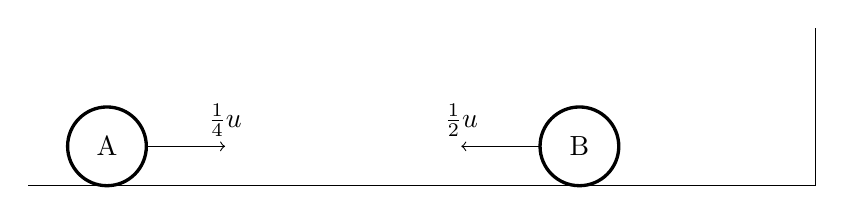
\begin{tikzpicture}
\filldraw[color=black,fill=none,very thick](3,0.5) circle (0.5) node{B};
\filldraw[color=black,fill=none,very thick](-3,0.5) circle (0.5) node{A};
\draw (-4,0) -- (6,0);
\draw (6,0) -- (6,2);
\draw[arrows=->](-2.5,0.5)--(-1.5,0.5) node[above]{$\frac{1}{4}u$};
\draw[arrows=->](2.5,0.5)--(1.5,0.5) node[above]{$\frac{1}{2}u$};
\end{tikzpicture}\\
\\
\textbf{Calculate the time it takes for B to approach the wall}\\
\\
\textcolor{red}{Time$=\dfrac{\text{Distance}}{\text{Speed}}$}\\
\\
\\
Time= $\dfrac{4a}{\frac{5}{4}u}=\dfrac{16a}{5u}$\\
\\
\textbf{Calculate the distance A moves towards the wall}\\
\\
$\text{Distance}=\dfrac{1}{4}u\times\dfrac{16a}{5u}=\dfrac{4}{5}a$\\
\\
\textbf{Calculate the speed A and B approach each other}\\
\\
$\dfrac{1}{4}u+\dfrac{1}{2}u=\dfrac{3}{4}u$\\
\\
\textbf{Calculate the distance between A and B immediately after B has collided with the wall}\\
\\
$4a-\dfrac{4}{5}a=\dfrac{16}{5}a$\\
\\
\textbf{Calculate time based on speed and distance}\\
\\
$t=\dfrac{\frac{16}{5}a}{\frac{3}{4}u}=\dfrac{64a}{15u}$\\
\\
\textbf{Add times to calculate total time}\\
\\
$\dfrac{16a}{5u}+\dfrac{64a}{15u}=\dfrac{112a}{15u}$
\newpage
\begin{center}
\underline{\huge Collisions example - Oblique Impact}
\end{center}
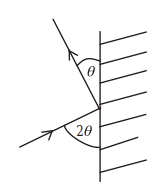
\includegraphics[width=1.5in]{oblique.png}\\
\\
\textit{A small smooth ball B, moving on a horizontal plane, collides with a fixed vertical wall.\\
Immediately before the collision the angle between the direction of motion of B and the wall is $2\theta$ where $0\degree < \theta < 45\degree$. Immediately after the collision the angle between the direction of motion
of B and the wall is $\theta$ as shown in the diagram above. Given that the coefficient of restitution
between B and the wall is $\frac{3}{8}$ , find the value of $\tan\theta$.}\\
\\
\textbf{Conservation of momentum}\\
\textcolor{red}{$m_1u_1=m_1v_1\Rightarrow u_1=v_1$}\\
\\
$u\cos2\theta=v\cos\theta$\\
\\
\textbf{Apply Newton's law of restitution}\\
\\
\textcolor{red}{$e=\dfrac{\text{Speed of separation}}{\text{Speed of approach}}$}\\
\\
$\dfrac{3}{8}=\dfrac{v\sin\theta}{u\sin2\theta}$\\
\\
\\
$3u\sin2\theta=8v\sin\theta$\\
\\
\textbf{Combine result from Conservation of Momentum and Restitution}




\end{document}